\chapter{Optimisation of ONT bioinformatics pipeline}\label{app_ONTBioinformatics}
\label{ONT_Bioinformatics_appendix}

\stoptocwriting
This section documents the results generated from processing ONT targeted datasets with various community-based tools and provides a rationale for the optimised ONT pipeline (depicted in XX) and the final curation of AD-associated transcripts in the mouse transcriptome (Chapter X). 

\subsection{Introduction}
As mentioned in \cref{section:ont_bioinformatics}, the bioinformatics pipeline for processing ONT raw reads was less defined and relied heavily on community-based tools particularly for the collapse and annotations of mapped ONT reads. These tools included:
\begin{enumerate}
	\item \textit{TAMA}, which allows collapsing long reads with a user-defined threshold for "wobble" (the maximum amount of bp difference between exon start sites and end sites across transcripts to be collapsed together) and comparison of annotated isoforms generated from different pipelines
	\item \textit{FLAIR}, which allows usage of genome annotations and/or short-read RNA-Seq splice junctions for correction of misaligned splice sites prior to collapse of long reads  
	\item \textit{TALON}, which also allows reference-based error correction was performed to remove microindels, mismatches and noncanonical splice junctions to generate a reference database. Each transcript from each sample is then compared to existing transcript models in this database, which is continually updated with incorporation of new transcript models where appropriate. \textit{TALON} further requires novel transcripts to be reproducibly detected across biological replicate samples 
\end{enumerate}
All three tools were trialled to process mapped ONT transcripts generated from enrichment of AD-associated genes in the rTg4510 mouse cortex for comprehensive isoform annotation and quantification. 

\subsection{Processing of ONT reads by \textit{TAMA} revealed necessity for splice-site error correction}
Usage of \textit{TAMA} for individual collapse and merging of each sample successfully curated thousands of full-length transcripts annotated to AD-associated genes, the vast majority of which were novel with novel splice-site junctions. 

The curated transcriptome was then further filtered with RNA-Seq data and using other parameters to remove artefacts from intra-priming, and reverse transcription template switching (as described in \cref{section: sqanti_annotations}). However, upon using RNA-Seq reads as junction support of isoforms with non-canonical junctions, the number of isoforms that were retained drastically fell from a total XXX isoforms annotated to AD target genes to XXX isoforms, with removal of all detected novel isoforms due to low short-read coverage (< 3 reads). Given the relatively high error rate of ONT reads (our ONT reads had an average 90\% accuracy (mean Phred Score = 10)), we suspected that many of the ONT reads had incorrectly sequenced splice sites, resulting in nan-canonical splice junctions that were not supported by RNA-Seq reads.


\subsection{Comparison of ONT and Iso-Seq datasets revealed insufficient coverage of RNA-Seq dataset}
We therefore performed a splice-site correction step using \textit{FLAIR}\cite{Tang2020}, which uses RNA-Seq reads to assess the validity of splice site boundaries: junctions supported by three uniquely mapping short-reads were considered valid, whereas incorrect splice sites were replaced with the nearest valid splice sites within a 10-nucleotide window - the final set of corrected reads only consist of reads with valid splice sites \cite{Tang2020}. Including this splice-site correction step after mapping with \text{Minimap2} and before isoform collapse with \textit{Tama}, we successfully recovered some novel transcripts. However, the usage of RNA-Seq reads for junction correction or support significantly reduced the final number of transcripts curated (XX to XX). 
% length and cage peak of those transcripts that are not supported 

We next compared the isoforms associated with target genes from all three ONT datasets generated either using RNA-Seq reads as support with \textit{SQANTI} or correction with \textit{FLAIR} and Iso-Seq dataset using \textit{Tama Merge} under default parameters. The vast majority of isoforms (99.8\%) detected using PacBio Iso-Seq were detected across all three ONT datasets. However, a third of Iso-Seq-derived isoforms overlapped with ONT-derived isoforms that were neither corrected with \textit{FLAIR} nor supported with RNA-Seq reads. This suggests that coverage of the RNA-Seq dataset at XX is insufficient to detect rare novel splice junctions and filtering of ONT reads with RNA-Seq dataset would be over-stringent with removal of true, novel, rare transcripts. Indeed, over 45\% of isoforms unique to ONT were filtered out, though the validity of these isoforms could not have been assessed. 

\begin{figure}[htp]
	\centering
	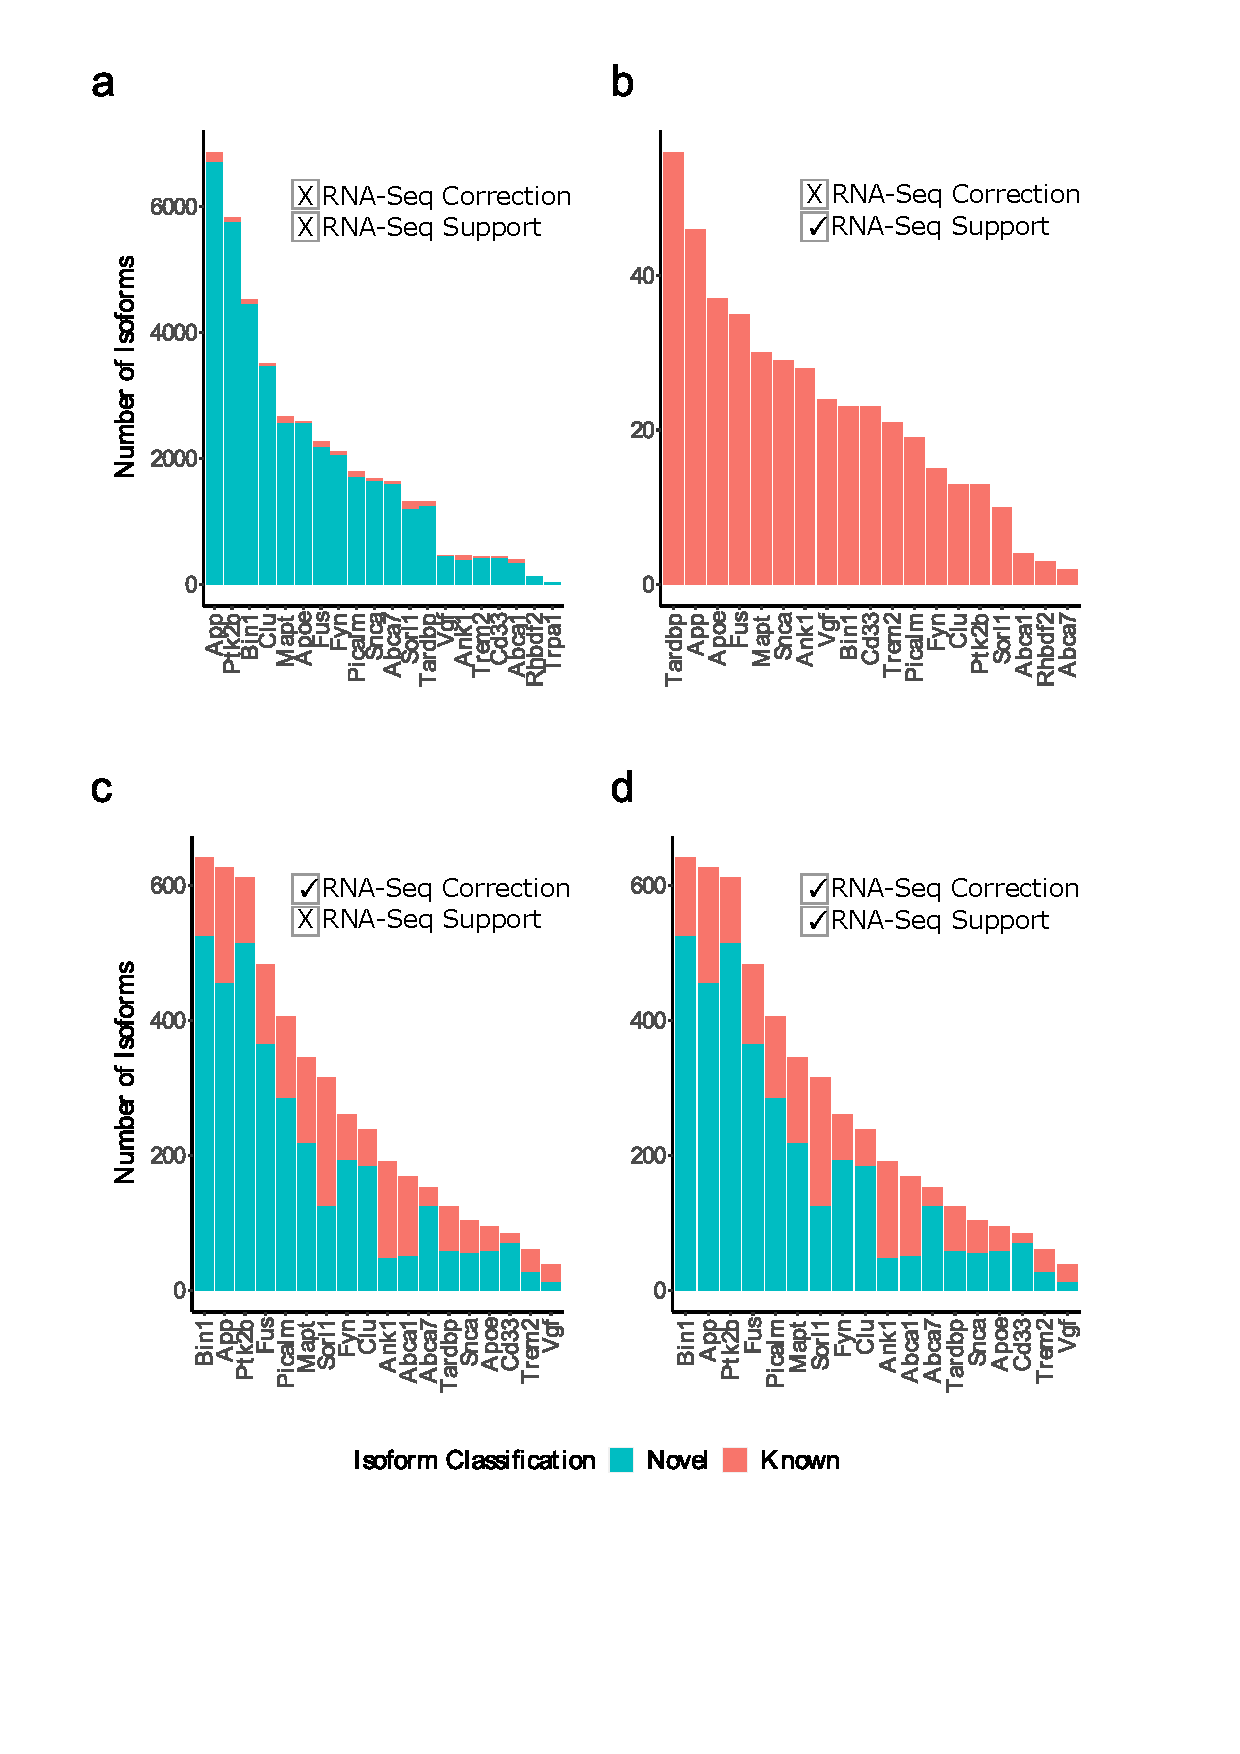
\includegraphics[page=1,trim={0cm 4cm 0cm 0cm},clip,scale = 0.8]{Figures/ONTTargetedTranscriptome_BioinformaticsPipeline}
	\captionsetup{width=0.95\textwidth,singlelinecheck=off}
	\caption[Number of ONT-derived isoforms associated with AD target genes using different bioinformatics approaches]%
	{\textbf{Number of ONT-derived isoforms associated with AD target genes using different bioinformatics approaches}. Shown is a bar chart of the final number of isoforms associated with AD target genes from ONT nanopore sequencing after \textit{SQANTI} annotation, using either RNA-Seq for splice junction correction with \textit{Flair} (RNA-Seq Correction) or RNA-Seq reads as junction support for (\textit{SQANTI} filter) (RNA-Seq Support) or both.   
	}
	\label{fig:ONT_bioinformatics}
\end{figure}

\begin{figure}[htp]
	\centering
	\includegraphics[page=2,trim={0cm 20cm 0cm 0cm},clip,scale = 0.65]{Figures/ONTTargetedTranscriptome_BioinformaticsPipeline}
	\captionsetup{width=0.95\textwidth,singlelinecheck=off}
	\caption[Overlap of isoforms associated with target genes detected using Iso-Seq and ONT sequencing]%
	{\textbf{Overlap of isoforms associated with target genes detected using Iso-Seq and ONT sequencing}. Shown is a venn diagram of the overlap of isoforms associated with AD target genes detected from ONT nanopore sequencing after \textit{SQANTI} annotation. ONT transcripts were corrected with RNA-Seq with \textit{Flair} (RNA-Seq Correction) or filtered out with RNA-Seq reads as junction support (\textit{SQANTI} filter) (RNA-Seq Support) or both. Of note, more samples were sequenced with the PacBio Iso-Seq approach (n = 24) than the ONT nanopore sequencing approach (n = 18).   
	}
	\label{fig:ONT_isoseq_comparisons}
\end{figure}

\subsection{Usage of TALON for appropriate correction and filtering of ONT reads}
\textit{TALON} was used to address the challenges of processing noisy ONT reads and achieve a balance between retaining true, novel rare transcripts and removing artefacts or novel transcripts that are not biologically meaningful. Rather than use RNA-Seq reads as filter, novel isoforms were removed if they were lowly-expressed and were not reproducibly detected as means of assessing transcript validity. Through this approach, we found that i) the majority of transcripts had only one read and were only detected in one sample, ii) the number of reads in each sample (expression) rather than the number of samples (reproducibility) primarily determine whether a transcript is retained or filtered, and ii) the default parameter (minimum 5 reads across minimum 2 samples) is too stringent in removing the vast majority of reads - a lower threshold (minimum 2 reads across minimum 2 samples) was therefore proposed. 

Notably, aside from the added features of reference-based error correction and quantification-led filtering, \textit{TALON} also superseded \textit{TAMA} and \textit{FLAIR} for simultaneous transcript discovery and quantification (the abundance output from \textit{TAMA}'s tama\_read\_support\_levels.py is computationally intensive to recover the read counts for each sample). 
\resumetocwriting